In this chapter, we introduce the problem of determining every location, here defined as the center and angle of rotation, of an ellipse with fixed shape parameters, such that it contains three given points.
This problem comes up in the development of an algorithm in \autoref{chapter:mcer} as a subproblem. Because no studies were found on it, or even on related problems, we decide to devote a whole chapter to presenting a handful of approaches we attempted, going through the issues with the failing ones, as well as discussing the qualities of the ones that shown to be successful.
In the end, we propose an algorithm for the problem that involves determining the eigenvalues of a $6\times6$ complex matrix. We also analyze its efficiency in terms of numerical accuracy and display some solutions that it was able to obtain.


\section{Definition}

We call the problem of finding a center and an angle of rotation for an ellipse given its shape parameters and three points that have to be on it \sigla{E3P}{Ellipse by Three Points}. An instance of it is given by three points $u, v, w \in \R^2$, along with the ellipse's shape parameters $(a, b) \in \R^2_{>0}$, with $a > b$.

Let $E: \R^2\times[0, \pi) \to \R^2$ be a function that takes the location of an ellipse with given shape parameters, and returns its coverage region as defined by \autoref{eq:rotated_ellipse_co}.
Then a solution of E3P can be defined as a pair $(q, \theta) \in \R^2\times[0, \pi)$, such that $\{u, v, w\} \subset \partial E(q, \theta)$. 

As a last remark, because of its application on \autoref{chapter:mcer}, a method would only be useful for our case if it can encounter every solution of E3P. This requirement makes the problem more challenging.

\section{Transforming the problem}\label{section:transforming-the-problem}

Initially, E3P is a problem with three unknown variables: the two coordinates of the ellipse's center point, $q_x$ and $q_y$, and the angle of rotation $\theta$. In this section, we transform E3P into the problem of finding the roots of a univariate function using a known circumcircle problem. 
This transformation, besides reducing the number of unknown variables to one, is later utilized in the demonstration that E3P has at most six distinct solutions.

To make the problem simpler, let us assume that point $u$ is at the origin. If it is not, a simple translation by $-u$ applied to the three points can be made to put $u$ at the origin.
Assume as well that $(q, \theta)$ is a solution of E3P, which means that an ellipse rotated by $\theta$, centered at $q$ contains $u$, $v$, and $w$ (see \autoref{fig:circumscribed-circle} for an example).
Taking this solution and applying a rotation of $-\theta$ to the coordinate system makes the ellipse become axis-parallel.
After that, we can transform that axis-parallel ellipse into a circle of radius $b$ by squeezing the $x$-axis by $\frac{b}{a}$. This two-step transformation can be written as a function $\varphi\colon \R^2 \to \R^2$ defined as

\begin{equation}\label{eq:trpnts}
\varphi(p, \theta)=\left[\begin{array}{cc}
\frac{b}{a}&0\\
0&1
\end{array}\right]
\left[\begin{array}{cc}
\cos{\theta}&\sin{\theta}\\
-\sin{\theta}&\cos{\theta}
\end{array}\right]\left[\begin{array}{c}
p_x\\
p_y
\end{array}\right].
\end{equation}
An example of this two-step transformation being applied to a solution of E3P is shown in \autoref{fig:circumscribed-circle}. 
Notice that $\varphi$ is a linear transformation. This means that given a final state, where after applying $\varphi$, the three points are on the radius-$b$ circle, a solution of E3P can be obtained by using the well-defined inverse function $\varphi^{-1}$.

Additionally, to make the notation more clear, we denote by $\Lambda(\theta)$ the triangle formed by the points $\varphi(u,\theta); \varphi(v, \theta); \varphi(w, \theta)$, as long as they are not collinear.
This being said, we can move forward and introduce a problem equivalent to E3P which is based on determining angles $\theta$ that make the triangle $\Lambda(\theta)$ be circumscribed in a circle of radius $b$.

\begin{figure}
	\centering
	\caption{Transforming a solution of E3P into a solution of the circumradius problem.}
	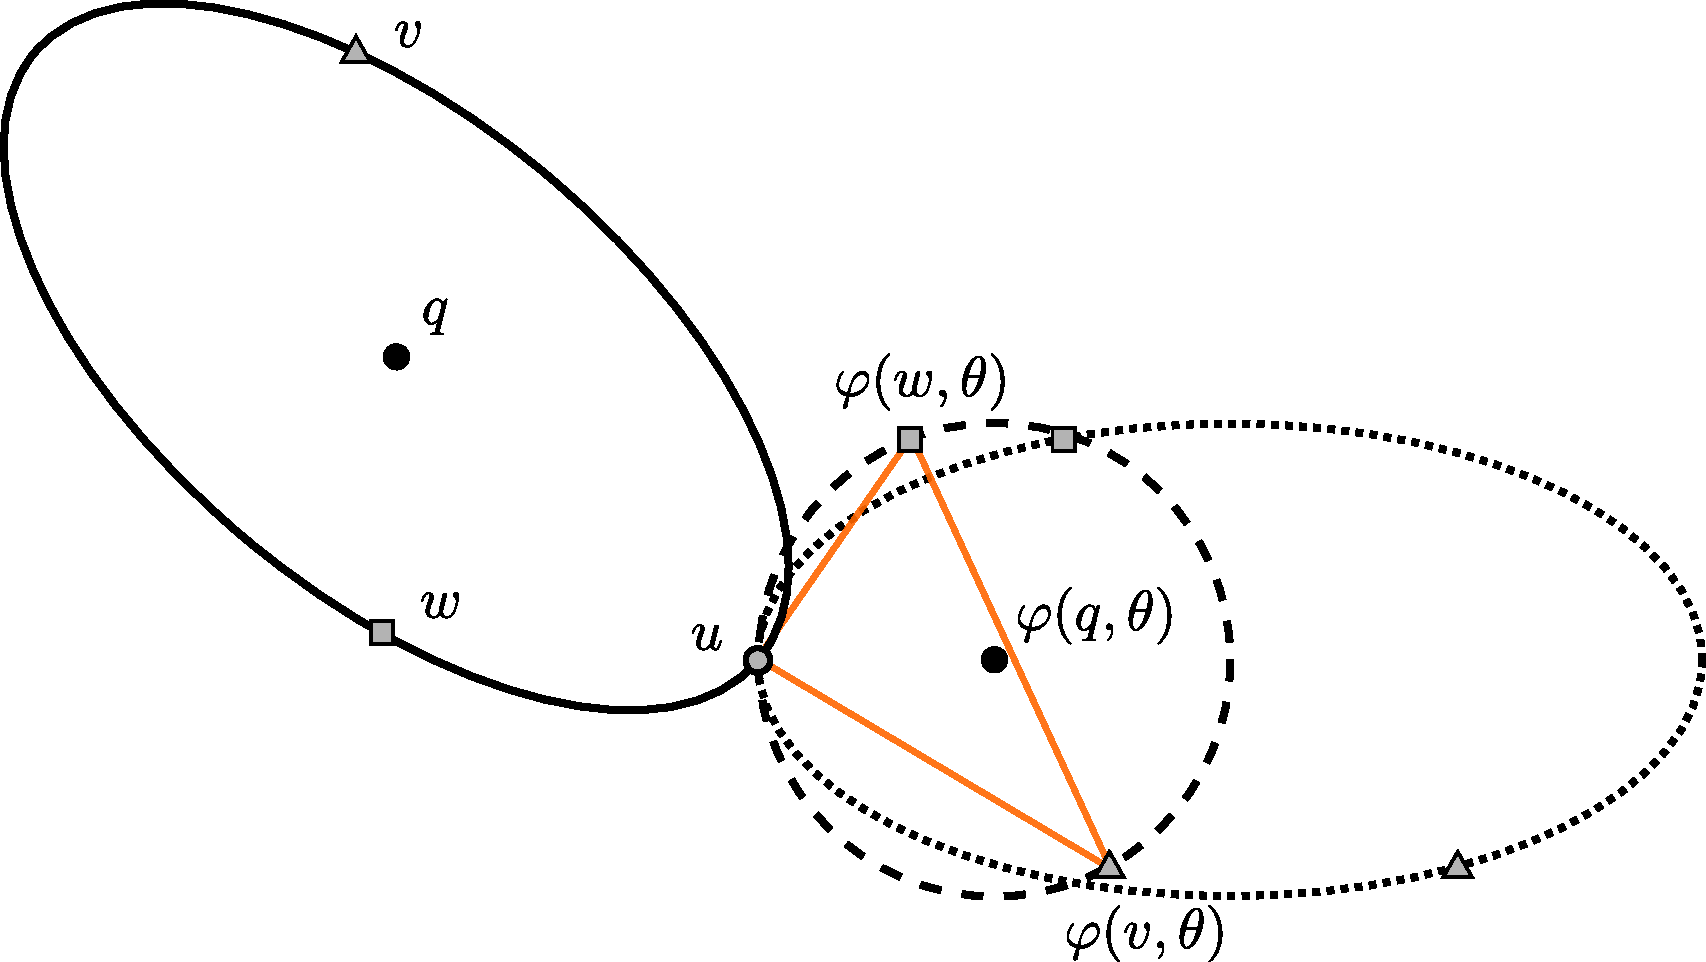
\includegraphics[scale=.4]{tex/figures/circumscribed-circle}
	\fautor
	\label{fig:circumscribed-circle}
\end{figure}

\subsection{A circumradius problem}

The term circumradius, in this work, is used to describe the radius of a triangle's circumscribed circle, which is a circle that contains the triangle's vertices. Given an instance of E3P, we define the circumradius problem as the problem of determining an angle $\theta\in[0, \pi)$, such that the circumradius of $\Lambda(\theta)$ is equal to $b$.

As it can be seen on \autoref{fig:circumscribed-circle}, given an instance of E3P and an angle of rotation $\theta\in[0, \pi)$ that makes $\Lambda(\theta)$ have a circumradius $b$, a solution for E3P can be obtained using the inverse transformation $\varphi^{-1}$. 
With that in mind, it is possible to conclude that both problems are equivalent because, from a solution of one, a unique solution of the other can be obtained.

The main reason to work with this problem is the reduction in the number of unknown variables from three to just one. This idea, however, would only be useful if checking the existence of a circumscribed circle with a radius $b$ given a triangle is a convenient problem.
It turns out that, for any triangle, there is always a unique circumscribed circle, which can be determined analytically. Given an instance of E3P and an angle of rotation $\theta \in [0, 2\pi]$, the circumradius $R$ of $\Lambda(\theta)$ can be computed through the following expression

\begin{equation}\label{eq:circumscribed_circle}
R = \dfrac{\norm{\varphi(v, \theta)}\norm{\varphi(w, \theta)}\norm{\varphi(v, \theta)-\varphi(w, \theta)}   }{4A(\theta)},
\end{equation}
with $A(\theta)$ being the area of $\Lambda(\theta)$ (for more details about \autoref{eq:circumscribed_circle}, or on how to determine the center of a circumscribed circle, see \citeonline[p.~189]{johnson1960}). It should be pointed out that this transformation does not preserve distance or area; if that was true, the radius defined by \autoref{eq:circumscribed_circle} would be constant.

With the formula for the circumradius in hands, a function can be defined, such that its roots provide solutions for the circumradius problem, and consequently, solutions for E3P.
Imposing the radius $R$ to be equal $b$ and squaring to eliminate the square roots present in the Euclidean distance, a function $\xi : [0, 2\pi) \mapsto \mathbb{R}_{>0}$ is defined as 
\begin{equation}\label{eq:circumscribed_circle_b}
\xi(\theta) = 16b^2A(\theta)^2 - \norm{\varphi(v, \theta)}^2\norm{\varphi(w, \theta)}^2\norm{\varphi(v, \theta)-\varphi(w, \theta)}^2.
\end{equation}
Any root of $\xi$ produces a triangle whose circumradius is $b$ and subsequently provides a solution for E3P. 

Before attempting to develop an algorithm to find every root of $\xi$, we address the question about the number of roots of $\xi$ in the interval $[0, \pi)$.

\subsection{The number of solutions of E3P}

One of the steps of the method developed in \autoref{chapter:mcer} is to iterate over every solution of E3P. Of course, doing that is only possible if E3P has a finite number of solutions. Moreover, even if the number of solutions is finite, discovering an upper-bound for that is essential for determining the algorithm's efficiency.

\begin{lema}\label{lema:e3p}
	Any instance of E3P has at most $6$ solutions.
\end{lema}

\begin{proof}
	
Back on \autoref{chapter:definitions}, real trigonometric polynomials were introduced. It was stated that any $n$-degree polynomial can have up to $2n$ distinct roots. It turns out that $\xi$ is a real trigonometric polynomial of degree $6$ and it can be written in the format given by \autoref{eq:trig_poly_2}. This implies that $\xi$ can have up to $12$ distinct roots.
 To show that, just note that it is possible to write $\norm{\varphi(v, \theta)}^2$ and $A(\theta)^2$ in the same form as given by \autoref{eq:trig_poly_2}:
 
 \begin{align}\label{eq:dd}
 	\norm{\varphi(v, \theta)}^2 = (v_x\frac{b}{a}\cos\theta + v_y\frac{b}{a}\sin\theta)^2 + (v_y\cos\theta - v_x\sin\theta)^2\\
 	\label{eq:dd2} A(\theta)^2=\dfrac{1}{4}\det\left(
 	\begin{array}{cc}
 		v_x\frac{b}{a}\cos\theta + v_y\frac{b}{a}\sin\theta&v_y\cos\theta - v_x\sin\theta\\
 		w_x\frac{b}{a}\cos\theta + w_y\frac{b}{a}\sin\theta&w_y\cos\theta - w_x\sin\theta
 	\end{array}\right)^2.
 \end{align}
  It is also possible to see that the term which has $\xi$'s highest degree is the multiplication of the three squared lengths of $\Lambda(\theta)$'s sides. This multiplication has the same degree of $(\norm{\varphi(v, \theta)}^2)^3$, and because $\norm{\varphi(v, \theta)}^2$ has degree $2$, the degree of $\norm{\varphi(v, \theta)}^2$ is $6$, which consequently is $\xi$'s degree.
Going from $12$ solutions to $6$ is done by using the symmetry of ellipses. In \autoref{chapter:definitions}, it was stated that any rotation in the interval $[0, \pi)$ is identical to a rotation in $[\pi, 2\pi)$. Because of that, half of the roots of $\xi$ are in $[\pi, 2\pi)$ and can be dismissed.
\end{proof}

\section{An attempt using the conic general equation}

The idea of this approach was to use the six-parameter conic equation to represent an ellipse. This equation is given by
\begin{equation}\label{eq:gen_ellipse}
Ax^2+Bxy+Cy^2+Dy+Ex+F=0,
\end{equation}
with $A, B, C, D, E,F \in \R$ being fixed parameters.
This equation actually represents any conic, for it to be an ellipse the condition $B^2 -4AC < 0$ must be satisfied.

Given an instance of E3P, assuming $u$ is at the origin, having that it satisfies \autoref{eq:gen_ellipse}, we get $F=0$. Using the other two points, it is possible to write $D$ and $E$ in terms of $A, B, C$. As any multiple of \autoref{eq:gen_ellipse} represents the same conic, we can set $B$ to be equal to $1$. Then, we end up with two variables, $A$ and $C$, and still need to impose that the final equation represents an ellipse with the given shape parameters. Let $\Delta=4AC-B^2=4AC-1$, and assume $F=0$, then the expressions for both major-axis and minor-axis, respectively are
\begin{align}\label{eq:gen_ellipse_a}
a^2 = \dfrac{2\dfrac{AE^2 -BDE +CD^2}{\Delta}}{A + C - \sqrt{1 + (A-C)^2}}\\
\label{eq:gen_ellipse_b}b^2 = \frac{2\dfrac{AE^2 -BDE +CD^2}{\Delta}}{A + C + \sqrt{1 + (A-C)^2}}.
\end{align}
These two equations define two curves in $\R^2$ with $A$ and $C$ being the chosen variables. The solutions lie in the set of intersection of these curves. This set can probably be approximated numerically, however, we decided not to further pursue this approach.

Another idea which has been explored was working with the ratio $\frac{a^2}{b^2}$, which becomes an expression that allows $A$ to be written as a function of $C$. At first, this function appeared to be monotonic, so we tried to develop a method based on that. However, cases where the function does not behave as nicely were found. It is likely that developing a method to approximate solutions working with this function is possible, but we decided not to continue on this track.


\section{An approximation method}

One of the most useful techniques when dealing with complicated functions is approximation. They appear in various methods whenever a derivative or integral needs to be calculated or, for example, like in our case, when the roots of a function need to be determined. In general, one has a function $f$ that is part of a family of functions $\mathcal{A}$ and wants to select a simpler function $f^*$ from a set of functions $\mathcal{A^*}$, such that $f^*$ is close enough to $f$ \cite[p.~3]{powell}. For this problem, we consider the approximation of $\xi$ on the interval $[0, \pi)$ by a function in the family of $n$-degree Chebyshev polynomials.

\subsection{Chebyshev polynomial}

Chebyshev polynomials are widely used in Numerical Analysis in areas like numerical integration, polynomial approximation, and ordinary and partial differential equations.
They are also very useful in practice and are present in extension libraries in Python, MATLAB and C.

Because of the scope of this work, only a brief introduction of Chebyshev polynomials of the first kind and its usage in polynomial interpolation is given. For a more thorough work on the subject, please check the book by \citeonline{chebbook}.

We refer to $T_n : [-1, 1] \mapsto [-1, 1]$ as the $n$-degree Chebyshev polynomial of the first kind, and it is defined as
\begin{equation}
T_n(x) = \cos({n\arccos (x)}).
\end{equation}
It is important to mention that this definition can be extended to the whole real line. Using some trigonometric identities, $T_n$ can also be expressed as a recurrence relation
\begin{equation}
T_n(x) = 2xT_{n-1}(x) - T_{n-2}(x).
\end{equation}

An important property worth bringing up is that Chebyshev polynomials are orthogonal and form a basis for the polynomial space. This implies that any $p_n$ of degree up to $n$ can be expressed as a truncated Chebyshev series
\begin{equation}\label{eq:chebseries}
p_n(x) = \sum_{j=0}^{n} a_j T_j(x).
\end{equation}

One of the greatest qualities of Chebyshev polynomials is their numerical stability. \citeonline{gautschi:1979} showed that the matrix that maps polynomials onto its coefficients written in the power form has a condition number that grows exponentially with $n$. On the other hand, the matrix that converts polynomials to the Chebyshev basis as \autoref{eq:chebseries} has a linear condition number bounded by $\sqrt{2}n$.

\subsection{Chebyshev interpolation}
Polynomial interpolation is a form of approximating a function by a polynomial of degree $n$ that passes through $n+1$ chosen points. In fact, this polynomial is unique and it is determined by Lagrange's formula
\begin{equation}\label{eq:lagrange}
f_n(x) = \sum_{j=0}^{n} f(x_j)\dfrac{\prod_{k \neq j}^{n+1} (x-x_k)}{\prod_{k \neq j}^{n+1} (x_j-x_k)},
\end{equation}
with $f$ being the function to be approximated, and $f_n$ the unique $n$-degree polynomial that passes through $\{(x_j, f(x_j)): j=0, 1, \dots n\}$. Because of the uniqueness of interpolant polynomials, there is a direct link between the quality of an approximation and the points chosen to interpolate. As a matter of fact, depending on the points one chooses, even increasing the degree of the interpolation makes the approximation worsen. This is known as Runge's phenomenon and an example can be seen in \citeonline[p.~37]{powell} where uniformly spaced points are chosen to interpolate the function $f(x) = (1+x^2)^{-1}$ on the interval $[-5, 5]$. 

That is where Chebyshev interpolation comes in. Instead of choosing $n+1$ arbitrary points, the $n+1$ roots of $T_{n+1}$, which are also known as Chebyshev Nodes, are chosen as the interpolation points. The $n+1$ Chebyshev Nodes are given by
\begin{equation}
x_j = \cos{\left(\dfrac{\pi(j-\frac{1}{2})}{n+1}\right)},
\end{equation}
for $j=1, \dots, n+1$. This particular choice defeats Runge's phenomenon and provides a convergent approximation. 
Note that, if the domain of the function to be interpolated is defined on a range other than $[-1, 1]$, let us say $[a, b]$, then the transformation
\begin{equation}
\hat{x_j} = \frac{a+b}{2} + \frac{b-a}{2}x_j
\end{equation}
can be done to map it to the Chebyshev Nodes' domain $[-1, 1]$.

Then, the Chebyshev interpolation of a function $f: [a, b] \mapsto \R$ can be determined using Lagrange's formula and the points $\hat{x}_1, \dots, \hat{x}_n$. 
As it was mentioned in \autoref{chapter:definitions}, finding the roots of a polynomial written in the monomial form can be done by determining the eigenvalues of a so-called Frobenius companion matrix. For small values of $n$ this works fine, however, converting the polynomial obtained by \autoref{eq:lagrange} to the power form, as $n$ grows, becomes a very ill-conditioned problem. 
An alternative method can be found in \citeonline{boyd:2013}, where the Chebyshev interpolation is calculated directly as a truncated Chebyshev series, as in \autoref{eq:chebseries}, in $\bigO(n^2)$. Also, given a polynomial written in the Chebyshev basis, a $n\times n$ matrix can be constructed, such that its eigenvalues are the roots of that polynomial. \citeonline{boyd:2013} refers to this matrix as the Chebyshev-Frobenius companion matrix.

Therefore, the whole process of interpolating and finding the roots can be done using only Chebyshev polynomials, which have great numerical stability. Also, Chebyshev-Frobenius matrices have the same property as companion matrices, which allows their eigenvalues to be found by a QR algorithm. Summing the two steps, a $\bigO(n^3)$ algorithm can be achieved, with $n$ being the degree of the interpolation.

The last question that needs to be addressed is: how close are the roots of the Chebyshev interpolant $f_n$ to the roots of $\xi$?

Even though $\xi$ is complicated enough, in a sense that finding its roots directly is no trivial task, it is a very well-behaved function: it is analytic and has infinitely many continuous and integrable derivatives. This satisfies all the requirements of the result in \citeonline[p.~28]{gottlieb}, which says that if a function has $m$ continuous and integrable derivatives in a closed interval, its absolute difference to its respective Chebyshev truncate series is $\bigO(n^{-m})$. Also, in \citeonline{battles:2004}, a theorem is presented stating that if a function is analytic on a neighborhood of $[-1, 1]$, then the convergence is $\bigO(C^n)$, for some $C<1$.

To choose the degree of the interpolation we use the last coefficient rule-of-thumb introduced by \citeonline[p.~50]{boyd:2001}. There is no guarantee that this method will choose $n$ such that $f_n$ is close enough to $\xi$ everywhere on $[0, \pi)$. Nonetheless, in practice, it is considered to be a good estimate for the error
\begin{equation}
r_n = \max_{0 \le \theta < \pi} |f_n(\theta) - \xi(\theta)|,
\end{equation}
which measures how far the interpolation is at the point it worst approximates. 
\clearpage
\subsection{Testing different interpolant degrees}

In this section, we describe the results of an experiment we made to verify the accuracy of solutions found by the Chebyshev Interpolation method for different interpolation degrees. 
The main reason for doing this experiment was to obtain a practical lower-bound for the interpolation degree, which can be used later to decide whether to use this method or not. We also investigate if dividing the interpolation interval into $K$ sub-intervals, which is a suggestion given in \citeonline{boyd:2013}, yields an improvement in the accuracy of solutions. 

We used the Python programming language in the implementation of this approach for E3P. More specifically, we utilized the external library SciPy, which has routines already implemented for Chebyshev interpolation, and finding the roots of a Chebyshev polynomial. More information about SciPy can be found in \cite{scipy}.
 
Let $\delta : \R^2 \to \R_{>0}$ be a function defined as the left-hand-side of \autoref{eq:rotated_ellipse}, then, for an instance of E3P with three points $u, v, w$, we define the error of a solution as $$\max\{|\delta(u)|, |\delta(v)|, |\delta(w)| \}.$$
We created instances of E3P taking every triplet of points, and every ellipse from an MCE's instance named CM3 proposed in \citeonline{canbolat}. We also tried dividing the interval $[0, \pi]$ into a different number of sub-intervals taking $K \in\{1, 2, 4, 8\}$.

\begin{figure}
	\centering
	\caption{The maximum interpolation error.}
	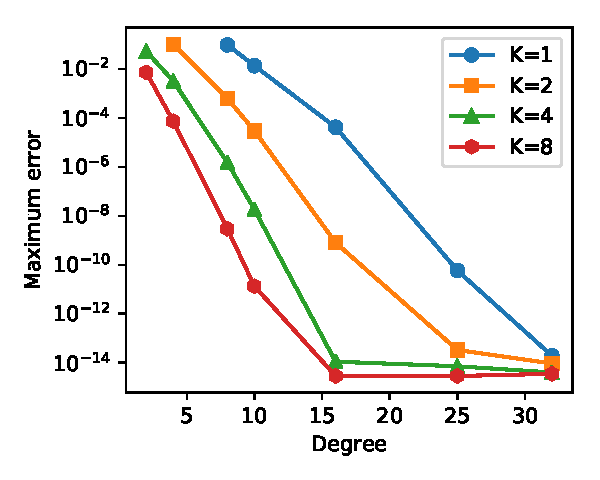
\includegraphics[scale=.9]{tex/figures/error_roots}
	\fautor
	\label{fig:interpolant_error}
\end{figure}

In \autoref{fig:interpolant_error}, for each $K$, the maximum error observed among every instance of E3P for each interpolation degree is shown. It may be stated that adopting the strategy of dividing the interpolation interval into $K$ sub-intervals provides a significant improvement in accuracy.

Also, as expected, in \autoref{fig:last-coeff}, using the same instances, we were able to observe that the maximum absolute value of the last coefficient among every instance has the same behavior as its corresponding error in \autoref{fig:interpolant_error}.

\begin{figure}
	\centering
	\caption{The maximum absolute value of the last coefficient interpolation.}
	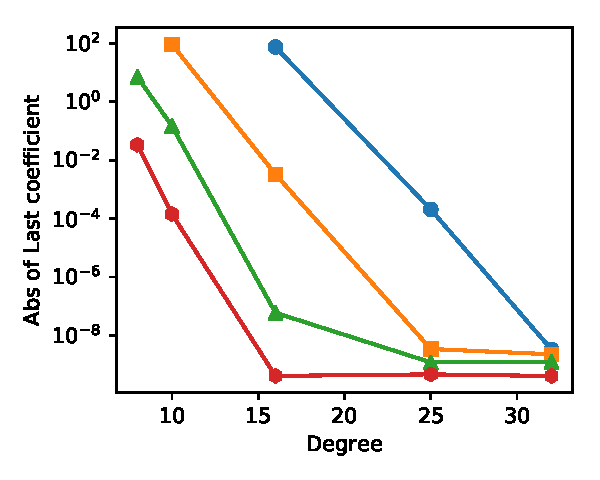
\includegraphics[scale=.9]{tex/figures/last_coeff}
	\fautor
	\label{fig:last-coeff}
\end{figure}

Assuming that $K=4$, we can say that for a small error to be achieved, we need to take an interpolation degree of at least $10$, increasing it based on the last coefficient rule. A suggestion in \citeonline{boyd:2013} says that if the last coefficient is not small, the interpolation degree must be doubled. 
This is only a suggestion of how to approach the problem of choosing a good interpolation degree. 
This procedure could still fail as a small last coefficient does not necessarily imply a small error everywhere in the interpolation interval. 

\section{Converting $\xi$ into a polynomial}

In \autoref{chapter:definitions}, a brief introduction is given on how to get the roots of a polynomial. For that reason, we discuss two ways of converting $\xi$ into a polynomial in this section. The first one converts $\xi$ into a real polynomial and the second one into a complex polynomial. For these two approaches we put symbolic computation into practice to obtain the coefficients of the polynomials in terms of the E3P's instance. 

%Symbolic computing was used to compute the polynomials, the Python external library called SymPy was utilized (see \citeonline{sympy} for more details).

\subsection{Real polynomial}

From $\xi$, a real polynomial can be obtained by using the identity $x = \tan{(\frac{\theta}{2})}$. We do not go in detail, but it is possible to show that a degree-$12$ polynomial can be obtained using that substitution.

%In practice, we utilized Python's external library SymPy (see \citeonline{sympy} for more details).

At first,  the root-finding algorithm described on \autoref{chapter:definitions} seemed to work fine and return every solution of E3P. However, we later found out that for some instances, priorly known roots were not being found. The cause was not for sure identified, but a good guess would be that for angles which are greater than $\frac{\pi}{4}$, $x$ starts growing too rapidly which could lead to numerical instability. This issue made us abandon this approach and pursue a different way to convert $\xi$ into a polynomial.

\subsection{Complex polynomial}

A complex polynomial can be obtained from $\xi$ by using an idea published in \citeonline{boyd:2006}. There, the author uses the identities

\begin{align}\label{eq:complex_trig_cos}
	\cos{(\theta)} &= \dfrac{e^{i\theta} + e^{-i\theta}}{2}\\
	\label{eq:complex_trig_sin}
	\sin{(\theta)} &= \dfrac{e^{i\theta} - e^{-i\theta}}{2i},
\end{align}
which relate complex numbers with trigonometric functions, to convert real trigonometric polynomials, which is the case of $\xi$, into univariate complex polynomials.
This approach is preferable as it preserves the numerical stability of the original real trigonometric polynomial -- more details about this can be found in \citeonline{weidner}, where it is stated that computing the roots of a real trigonometric polynomial through this transformation does not yield loss of accuracy.

It is possible to show that with that substitution and changing the variable to $z=e^{i\theta}$, we obtain the following function $g : \mathbb{S} \mapsto \mathbb{C}$, with $\mathbb{S}$ being the unit complex circle ($\mathbb{S} = \{z \in \mathbb{C} : |z|=1\}$):

\begin{equation}
g(z)=\sum_{k=0}^{12} c_k z^{k-6},
\end{equation}
for some $c_0, \dots, c_{12} \in \mathbb{C}$. As the equalities on \autoref{eq:complex_trig_cos} and \autoref{eq:complex_trig_sin} are valid for any $\theta \in \R$, function $g(e^{i\theta})$ and $\xi$ are equivalent, since $g(e^{i\theta}) = \xi(\theta)$ for any $\theta \in [0, 2\pi]$. Notice that $g$ is not a complex polynomial it has negative exponents and its domain is not $\mathbb{C}$.

We can get rid of negative exponents by multiplying $g$ by $z^6$. This does not create further problems as $0\not\in \mathbb{S}$. The second issue is removed by simply extending the domain from $\mathbb{S}$ to $\mathbb{C}$. 
As $\mathbb{S} \subset \mathbb{C}$, roots outside the unit circle could appear in the new polynomial, but they can be ignored as they are not roots of $g$.
Finally, from $g$, the polynomial $h : \mathbb{C} \mapsto \mathbb{C}$ is defined as

\begin{equation}\label{eq:h}
h(z) = z^6 g(z) = \sum_{k=0}^{12} c_k z^k.
\end{equation}
By its definition it is possible to see that every root of $g$ is also a root of $h$, and conversely, every root of $h$ which is in $\mathbb{S}$, is also a root of $g$. Lastly, every root of $g$ will correspond to a root of $\xi$ through their angles on the unit circle.

\subsubsection{Further improvements}

It is possible to make another reduction and cut the size of the polynomial in half.
As it has been mentioned in \autoref{chapter:definitions}, an ellipse is symmetric with respect to its axis, which implies that rotating it by $\theta \in [0, \pi)$ is equivalent to rotating it by $\pi + \theta$.
On the other hand, very conveniently, as given by \autoref{eq:angle_op_sign}, angles of complex numbers of opposite signs are $\pi$ apart from each other, which means that $g$ has to produce the same output for both $z$ and $-z$ as they represent equivalent angles of rotation for ellipses.
From that, for all $z\in \mathbb{S}$ we have
\begin{align*}
h(-z) = (-z)^6g(-z) = z^6g(z) = h(z).
\end{align*}
Therefore, every odd degree coefficients of $h$ must be zero and we can define the $6$-degree polynomial $f : \mathbb{C} \mapsto \mathbb{C}$ with the substitution $y=z^2$ as follows
\begin{equation}\label{eq:poly_f}
f(y) = \sum_{k=0}^{6} c_{2k} y^k.
\end{equation}
Then from every root $\hat{y}$ of $f$, two roots of $h$ can be obtained: $\sqrt{\hat{y}}$ and $-\sqrt{\hat{y}}$. As the angle of one of the roots will not be between $[0, \pi)$ we can ignore one of them. 
Note that the square root of $\hat{y}$ does not need to be calculated, as only the angles are needed and they can be obtained by the identity
\begin{equation*}
angle(\sqrt{z}) = angle(z)/2.
\end{equation*}

It is also worth mentioning that a pattern on the coefficients of $f$ was identified, and maybe, for future work, it can be used for further improvements. Analyzing the polynomials produced for several instances, the following seems to be true:
\begin{equation}\label{eq:palindromic_pol}
c_k = \overline{c_{6-k}},
\end{equation}
for $k=0, \dots, 6$. For now, we neither have any ideas on how \autoref{eq:palindromic_pol} could be proved nor how it could be used to find the roots of $f$.

Finally, in the next section we use this approach of converting $\xi$ into a complex polynomial to develop an algorithm for E3P.

\section{An algorithm for E3P}

Among the methods that have been described here, converting $\xi$ into a complex polynomial, and then obtaining its roots by determining the eigenvalues of a companion matrix was the chosen one as the basis of \autoref{algoritmo:e3p} for E3P.
Despite the good results shown by the Chebyshev interpolation method,
it can still be classified as a heuristic as none of the approaches to determine the interpolation degree ensures a good approximation in the whole interval.
On top of that, ultimately, the roots of the Chebyshev polynomial are computed through determining the eigenvalues of a companion matrix, which, unless a lower-than-seven interpolation degree is utilized, is going to be larger than the companion matrix whose eigenvalues are the roots of the complex polynomial $h$.

Details about getting the eigenvalues of a companion matrix, and determining the center of a circumscribed circle of a triangle are omitted from \autoref{algoritmo:e3p} for the sake of clarity. 
In our implementation, we use symbolic computation to determine the coefficients of $h$ in terms of the parameters of a E3P's instance. This way, we only need to compute once separately from the main algorithm. We get into more detail about that in \autoref{chapter:numerical}.

Having all the coefficients of $h$ available, basically, after building a companion matrix, \autoref{algoritmo:e3p} applies the reverse transformations described by \autoref{eq:trpnts} to every eigenvalue of that companion matrix to obtain a solution for E3P.

\begin{algoritmo}
	\caption{Algorithm for E3P.}\label{algoritmo:e3p}
	\begin{algorithmic}[1]
		\Require{$u, v, w\in\R^2$, and $a, b\in\R_{>0}$, with $a>b$.}
		\Ensure{Every solution of E3P.}
		
		\item[]
		
		\Procedure{$e3p$}{$u,v,w,a,b$}
		
		\State $\hat{u}\gets (0,0)$ \Comment{Translate the system, so $u$ is at the origin.}
		\State $\hat{v} \gets v-u$
		\State $\hat{w} \gets w-u$
		
		\State Let $c_0, \dots, c_{12}$ be the coefficients of polynomial $h$ as \autoref{eq:h}.
		\State Let $A$ be a $6\times6$ zero matrix.
		
		\For{$i\in\{1, \dots, 6\}$}\Comment{Constructing the companion matrix.}
			\State $A_{i,i+1} \gets 1$
			\State $A_{6,i} \gets -\dfrac{c_{2(i-1)}}{c_{12}}$
		\EndFor

		
		\State $Q \gets \{\}$
		
		\ForAll{$q \in eig(A)$} \Comment{$eig(A)$ returns every eigenvalue of $A$.}
		\State $\theta\gets \min\{angle(-q)/2, angle(q)/2\}$
		\If{$|\theta|=1$}
			\State Let $c$ be the center of the circumscribe circle of $\Lambda(\theta)$.
			\State $Q \gets Q\cup \{(\varphi^{-1}(c, \theta)+u, \theta)\}$
		\EndIf
		\EndFor
				
		\State \Return $Q$
		\EndProcedure
	\end{algorithmic}
\end{algoritmo}

\begin{theorem}\label{th:e3p}
	\autoref{algoritmo:e3p} computes every solution for an instance of E3P in $\bigO(1)$ operations.
\end{theorem}

\begin{proof}
	It has already been shown in Section~\ref{section:transforming-the-problem} that computing every root of $\xi$ through the complex polynomial yields every solution of E3P. The only thing left to prove is the running time of the algorithm.
	Computing every eigenvalue of a matrix can be done in $\bigO(n^3)$, but as for our case $n$ is fixed at $6$, it can be stated that computing the eigenvalues for the companion matrix of $f$ can be done in $\bigO(1)$.
\end{proof}

\subsection{Instances with six and four solutions}

Any instance of E3P, as stated by \autoref{lema:e3p} can have up to six solutions. At first, though, this bound seemed to be loose as for randomly generated instances like the ones generated by the model in the next section, only two solutions were returned by \autoref{algoritmo:e3p}.
After some investigation, we were able to construct some four-solution instances (an example is displayed in \autoref{fig:e3p_4sols}). An interesting property of those solutions is that every one of them has their three points form an isosceles triangle.

\begin{figure}[H]
	\centering
	\caption{An instance of E3P with four solutions.}
	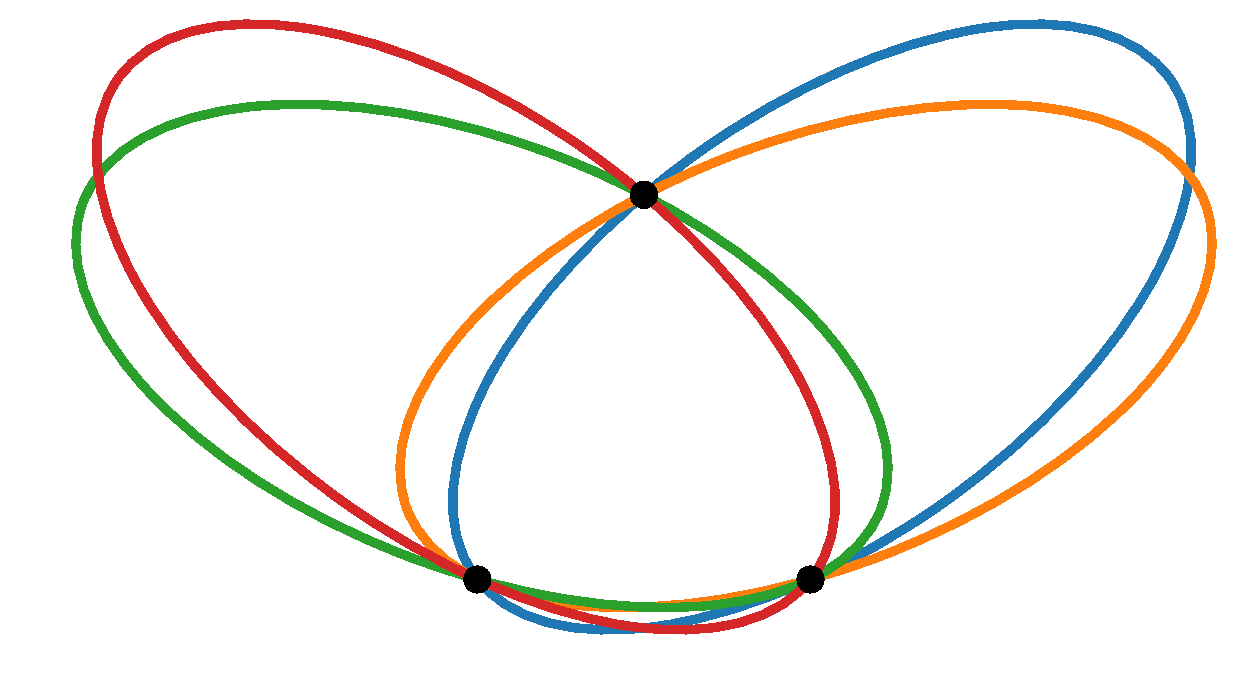
\includegraphics[scale=.33]{tex/figures/e3p_4sols}
	\fautor
	\label{fig:e3p_4sols}
\end{figure}

Obtaining six-solution instances, on the other hand, was done by taking a particular case of the isosceles-triangle approach.
As it can be seen in \autoref{fig:e3p_6sols}, the three points on every one of the six ellipses' border form an equilateral triangle. 

\begin{figure}
	\centering
	\caption{An instance of E3P with six solutions.}
	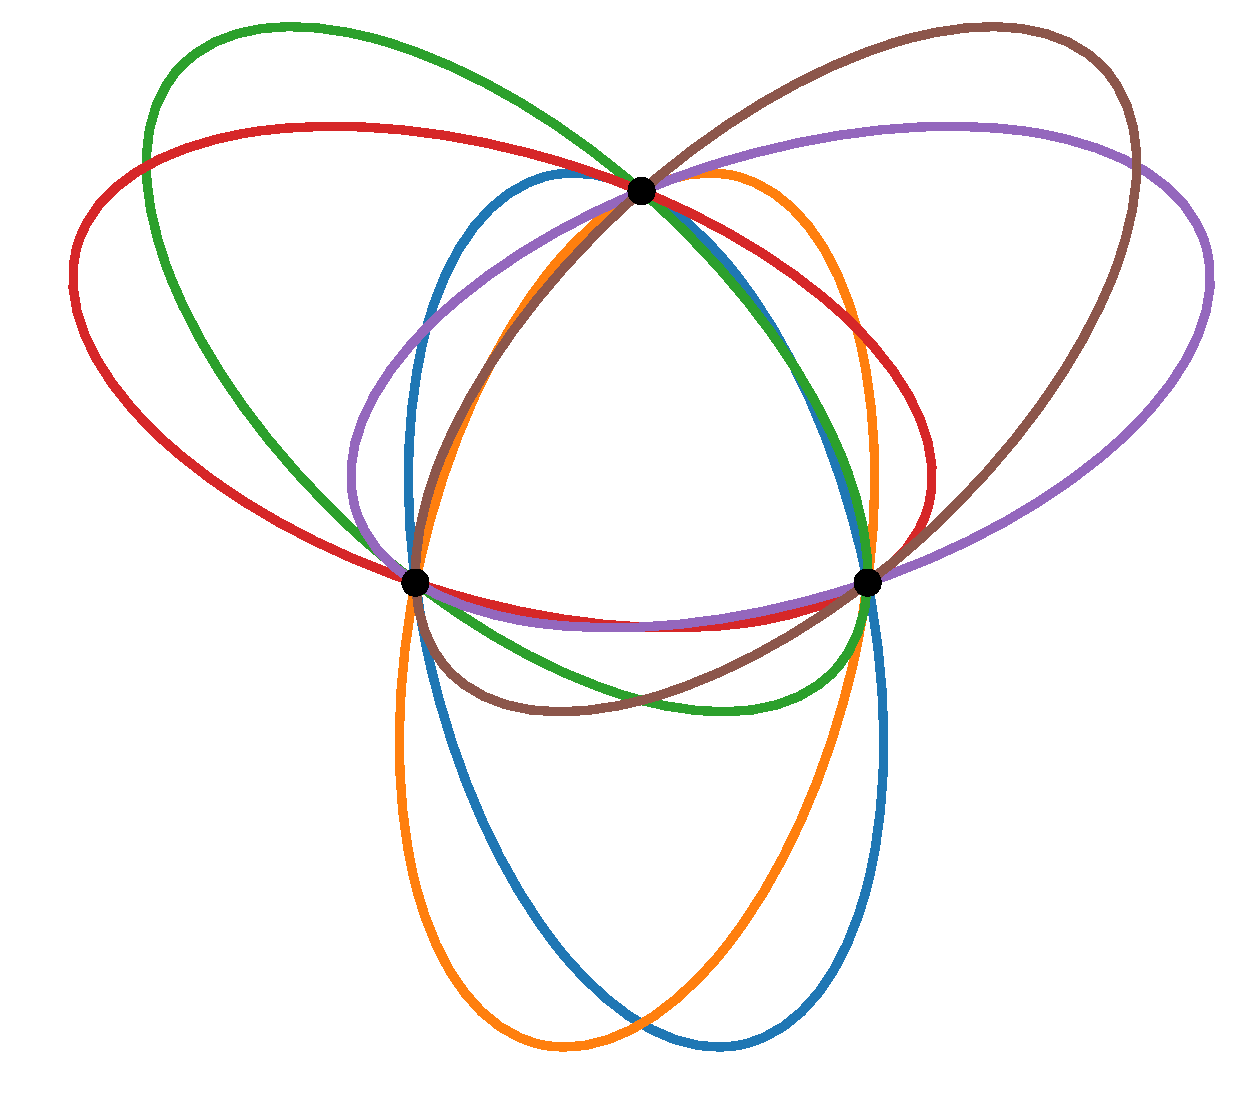
\includegraphics[scale=.33]{tex/figures/e3p_6sols}
	\fautor
	\label{fig:e3p_6sols}
\end{figure}

It should be pointed out that neither non-isosceles instances with four solutions nor non-equilateral instances with six solutions could be found. Further investigating these possible properties of E3P is left as future work.


\subsection{Numerical Stability}

In this section we show the results of some experiments made to study the numerical stability of \autoref{algoritmo:e3p}. For all the experiments, we define $K\in\R_{>0}$, and consider instances with ellipse's shape parameters $(K, \frac{K}{2})$, for $K\in\{10^j\colon j=0,\dots,10\}$. Let $\delta\colon\R^2\to\R$ be a function defined as the left-hand-size of \autoref{eq:rotated_ellipse}, then, for an instance with three points $u, v, w \in \R^2$, we define the error associated with a solution for that instance as $\max\{|\delta(u)|, |\delta(v)|, |\delta(w)|\}$.

The first experiment considers instances where the three points are the vertices of an ellipse rotated by $\theta\in[0, \pi)$. It is possible to see that such instances only have one solution, and therefore, roots with multiplicity greater than one are expected, which can be seen as a special case. 
For each value of $K$, we ran the algorithm for $100$ instances generated randomly by sampling $\theta$ according to a uniform distribution. For each instance, we took the closest solution to the priorly known one, and then, for each $K$, as it can be seen in \autoref{fig:e3p_known_sols1}, we considered the maximum and the average error.
\begin{figure}[H]
	\centering
	\caption{The maximum and average error for instances with known solutions.}
	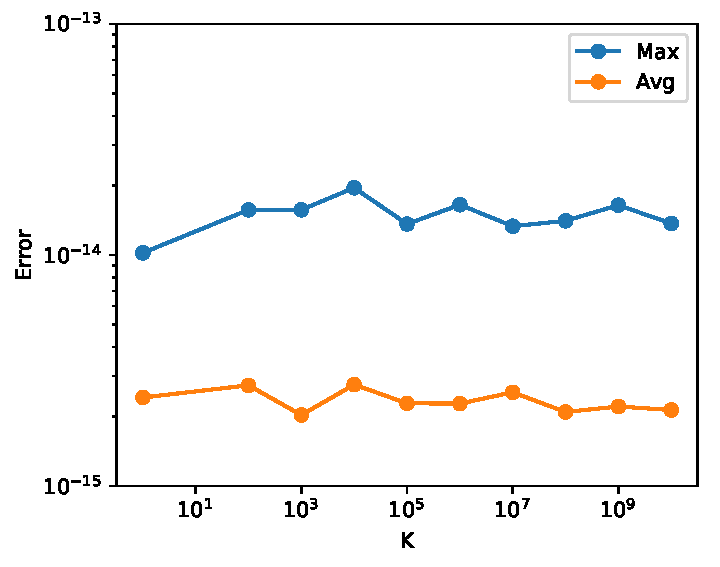
\includegraphics[scale=.75]{tex/figures/e3p_known_sols1}
	\fautor
	\label{fig:e3p_known_sols1}
\end{figure}
The second experiment takes the same instances as the previous one, but this time, we analyze how close the roots corresponding to the priorly known solutions are to the unit circle. The distance of a root $\hat{x}$ of $h$ to the unit circle is taken to be $|\hat{x}-1|$. This experiment is utilized mostly to determine a good precision constant for floating point comparisons in the implementation. The results are shown in \autoref{fig:e3p_known_sols2}. As it can be seen that the distance always stays under $10^{-6}$ we concluded that a good precision constant would be $10^{-5}$.
\begin{figure}
	\centering
	\caption{The distance of the roots to the unit circle.}
	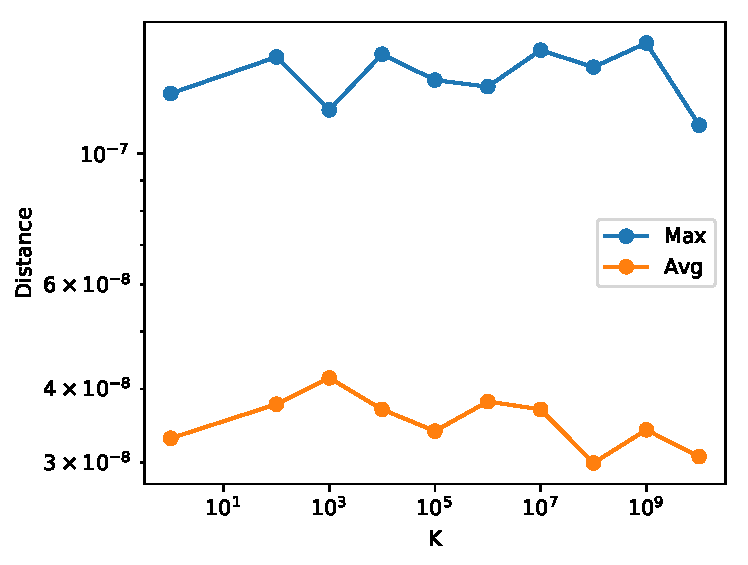
\includegraphics[scale=.75]{tex/figures/e3p_known_sols2}
	\fautor
	\label{fig:e3p_known_sols2}
\end{figure}

For the last experiment we considered $100$ instances for each $K$ with three points $(K\cos(t_j), \frac{K\sin{(t_j)}}{2})$, $j=1\dots3$, generated randomly by sampling $t_j$ according to a uniform distribution in $[0, 2\pi]$. The average and the maximum error are plotted in \autoref{fig:e3p_error}, and analyzing it, it is fair to say that \autoref{algoritmo:e3p} is numerically stable for this example, and its error, in average, is expected to be small even if the instance's numerical values are big.
\begin{figure}[H]
	\centering
	\caption{The error measured on solutions found by \autoref{algoritmo:e3p}.}
	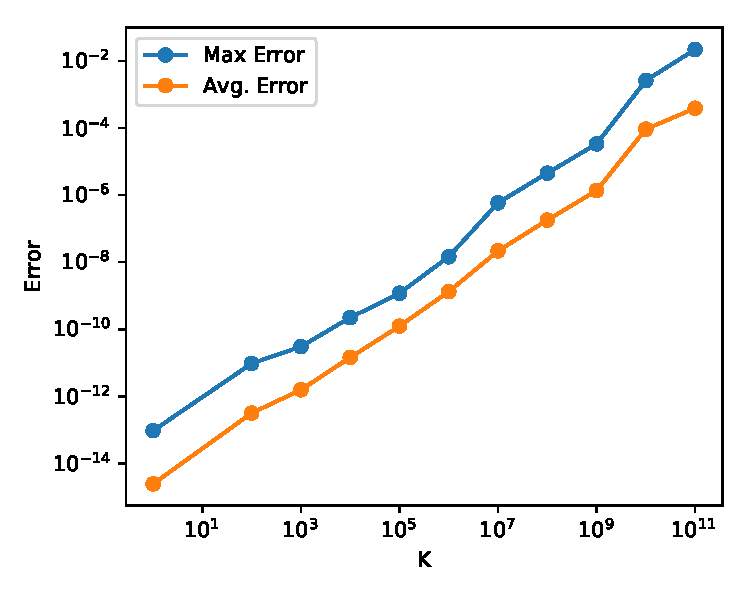
\includegraphics[scale=.75]{tex/figures/e3p_error}
	\fautor
	\label{fig:e3p_error}
\end{figure}
